\section{Advanced Operations}
\label{sec:advanced_operations}

\subsection{Intersect}

The intersection of two acceptors is the set of strings which is accepted by
both of them. The score of a path in the intersected graph is the sum of the
score of the path in each of the input graphs. More formally the language of
the intersected graph is given by $\{ \vx \mid \vx \in \L(\gA_1) \;\land\; \vx
\in \L(\gA_2)\}$.

The analagous operation for transducers is the composition, which we will
discuss in more detail in the next section. In most machine learning
applications, intersect and compose tend to be the primary operations used to
compute more complex graphs from simpler input graphs. Thus gaining a deeper
understanding of these two operations is worth the time.

We'll use the two graphs in figure~\ref{fig:intersect_inputs} to illustrate a
general algorithm for computing the intersection. In this case, the intersected
graph is easy to see by inspecting the two graphs. The only string which is
recognized by both graphs is the string $ab$, hence the intersected graph is
the graph which recognizes $ab$.

\begin{figure}
    \centering
    \begin{subfigure}[b]{0.48\textwidth}
        \centering
        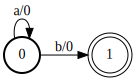
\includegraphics[scale=\dotscale]{figures/intersect_1}
    \end{subfigure}
    \begin{subfigure}[b]{0.48\textwidth}
        \centering
        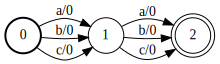
\includegraphics[scale=\dotscale]{figures/intersect_2}
    \end{subfigure}
    \caption{The acceptor on the left has a language of $a^*b$ and the acceptor
    on the right accepts all nine sequences of lenght $2$. The only sequence
    accepted by both, and hence is in the intersection, is the string $ab$.}
    \label{fig:intersect_inputs}
\end{figure}

The general algortihm relies on a queue to explore pairs of states from the two
input graphs. Pseudocode is given in algorithm~\ref{alg:intersect}.

\begin{algorithm}[t]
\caption{Intersect}
\label{alg:intersect}
\begin{algorithmic}[1]
\STATE \textbf{Input}: Acceptors $\gA_1$ and $\gA_2$
\STATE Initialize the queue $Q$ and the intersected graph $\gI$.

\FOR {$s_1$ and $s_2$ in all start state pairs of $\gA_1$ and $\gA_2$}
    \STATE Add $(s_1, s_2)$ to $Q$ and as a start state in $\gI$.
    \IF {$s_1$ and $s_2$ are accept states}
        \STATE Make $(s_1, s_2)$ an accept state in $\gI$.
    \ENDIF
\ENDFOR

\WHILE {$Q$ is not empty}
    \STATE Remove the next state pair $(u_1, u_2)$ from $Q$.
    \FOR {all arcs pairs $a_1$ and $a_2$ leaving $u_1$ and $u_2$ with matching labels}
        \STATE Get destination states $v_1$ of $a_1$ and $v_2$ of $a_2$.
        \IF {not yet seen $(v_1, v_2)$}
            \STATE Add $(v_1, v_2)$ as a state to $\gI$ and to $Q$.
            \IF {$v_1$ and $v_2$ are accept states}
                \STATE Make $(v_1, v_2)$ an accept state in $\gI$.
            \ENDIF
        \ENDIF
        \STATE Get the label $\ell$ of $a_1$.
        \STATE Get the weights $w_1$ of $a_1$ and $w_2$ of $a_2$.
        \STATE Add an arc from $(u_1, u_2)$ to $(v_1, v_2)$ with label $\ell$
        and weight $w_1 + w_2$.

    \ENDFOR
\ENDWHILE
\STATE \textbf{Return}: The intersected graph $\gI$.
\end{algorithmic}
\end{algorithm}


Some of the steps of the intersect algorithm on the two input graphs in
figure~\ref{fig:intersect_inputs} are shown in the sequence of graphs in
figure~\ref{fig:intersect_steps}. The states explored at each step are
highlighted in red. The intersected graph is the third graph on the right which
is constructed over the steps of the algorithm.

\begin{figure}
    \begin{subfigure}{\linewidth}
        \begin{minipage}{0.22\textwidth}
            \centering
            \includegraphics[scale=\dotscale]{figures/intersect_step_1_g1}
        \end{minipage}
        \begin{minipage}{0.37\textwidth}
            \centering
            \includegraphics[scale=\dotscale]{figures/intersect_step_1_g2}
        \end{minipage}
        \begin{minipage}{0.37\textwidth}
            \centering
            \includegraphics[scale=\dotscale]{figures/intersect_step_1_g_out}
        \end{minipage}
        \caption{The starts states in the input graphs are $0$ and $0$. So we
        add the start state $(0, 0)$ to the intersected graph and to the queue
        to be explored.}
    \end{subfigure}

    \begin{subfigure}{\linewidth}
        \begin{minipage}{0.22\textwidth}
            \centering
            \includegraphics[scale=\dotscale]{figures/intersect_step_2_g1}
        \end{minipage}
        \begin{minipage}{0.37\textwidth}
            \centering
            \includegraphics[scale=\dotscale]{figures/intersect_step_2_g2}
        \end{minipage}
        \begin{minipage}{0.37\textwidth}
            \centering
            \includegraphics[scale=\dotscale]{figures/intersect_step_2_g_out}
        \end{minipage}
        \caption{The first pair of outgoing arcs match on the label $a$. This
        means the downstream state $(0, 1)$ is reachable in the intersected
        graph. So we add $(0, 1)$ to the intersected graph and to the queue to
        be explored.}
    \end{subfigure}

    \begin{subfigure}{\linewidth}
        \begin{minipage}{0.22\textwidth}
            \centering
            \includegraphics[scale=\dotscale]{figures/intersect_step_3_g1}
        \end{minipage}
        \begin{minipage}{0.37\textwidth}
            \centering
            \includegraphics[scale=\dotscale]{figures/intersect_step_3_g2}
        \end{minipage}
        \begin{minipage}{0.37\textwidth}
            \centering
            \includegraphics[scale=\dotscale]{figures/intersect_step_3_g_out}
        \end{minipage}
        \caption{The next matching pair of outgoing arcs match on the label
        $b$. Also, we haven't visited the downstream state $(1, 1)$ yet. So we
        add $(1, 1)$ to the intersected graph and to the queue to be explored.}
    \end{subfigure}

    \begin{subfigure}{\linewidth}
        \begin{minipage}{0.22\textwidth}
            \centering
            \includegraphics[scale=\dotscale]{figures/intersect_step_4_g1}
        \end{minipage}
        \begin{minipage}{0.37\textwidth}
            \centering
            \includegraphics[scale=\dotscale]{figures/intersect_step_4_g2}
        \end{minipage}
        \begin{minipage}{0.37\textwidth}
            \centering
            \includegraphics[scale=\dotscale]{figures/intersect_step_4_g_out}
        \end{minipage}
        \caption{The arc in the second input graph with label $c$ does not have
        a matching arc from state $0$ in the first input graph, so it is
        ignored.}
    \end{subfigure}

    \begin{subfigure}{\linewidth}
        \begin{minipage}{0.22\textwidth}
            \centering
            \includegraphics[scale=\dotscale]{figures/intersect_step_5_g1}
        \end{minipage}
        \begin{minipage}{0.37\textwidth}
            \centering
            \includegraphics[scale=\dotscale]{figures/intersect_step_5_g2}
        \end{minipage}
        \begin{minipage}{0.37\textwidth}
            \centering
            \includegraphics[scale=\dotscale]{figures/intersect_step_5_g_out}
        \end{minipage}
        \caption{At this point we have considered all the matching outgoing
        arcs from $(0, 0)$ so we now move on to the next state pair in the
        queue, $(0, 1)$. From $(0, 1)$, a pair of outgoing arcs match on the
        label $a$. The downstream state $(0, 2)$ is new so we add it to the
        intersected graph and to the queue.}
    \end{subfigure}

\end{figure}

\begin{figure}\ContinuedFloat
    \begin{subfigure}{\linewidth}
        \begin{minipage}{0.22\textwidth}
            \centering
            \includegraphics[scale=\dotscale]{figures/intersect_step_6_g1}
        \end{minipage}
        \begin{minipage}{0.37\textwidth}
            \centering
            \includegraphics[scale=\dotscale]{figures/intersect_step_6_g2}
        \end{minipage}
        \begin{minipage}{0.37\textwidth}
            \centering
            \includegraphics[scale=\dotscale]{figures/intersect_step_6_g_out}
        \end{minipage}
        \caption{The next pair of matching outgoing arcs match on the label $b$
        and lead to the state pair $(1, 2)$. We add $(1, 2)$ to the queue and
        to the interescted graph. Also, since $1$ is an accept state in the
        first graph and $2$ is an accept state in the second graph, $(1, 2)$ is
        an accept state in the intersected graph.}
    \end{subfigure}

    \begin{subfigure}{\linewidth}
        \begin{minipage}{0.22\textwidth}
            \centering
            \includegraphics[scale=\dotscale]{figures/intersect_step_7_g1}
        \end{minipage}
        \begin{minipage}{0.37\textwidth}
            \centering
            \includegraphics[scale=\dotscale]{figures/intersect_step_7_g2}
        \end{minipage}
        \begin{minipage}{0.37\textwidth}
            \centering
            \includegraphics[scale=\dotscale]{figures/intersect_step_7_g_out}
        \end{minipage}
        \caption{Again, the arc in the second input graph with label $c$ does
        not have a matching arc from state $0$ in the first input graph, so it
        is ignored.}
    \end{subfigure}

    \begin{subfigure}{\linewidth}
        \begin{minipage}{0.22\textwidth}
            \centering
            \includegraphics[scale=\dotscale]{figures/intersect_step_8_g1}
        \end{minipage}
        \begin{minipage}{0.37\textwidth}
            \centering
            \includegraphics[scale=\dotscale]{figures/intersect_step_8_g2}
        \end{minipage}
        \begin{minipage}{0.37\textwidth}
            \centering
            \includegraphics[scale=\dotscale]{figures/intersect_step_8_g_out}
        \end{minipage}
        \caption{The next state pair in the queue is $(1, 1)$. There are no
        arcs leaving state $1$ in the first input graph, and $(1, 1)$ is not an
        accept state in the intersected graph, so it is a dead end. We can
        remove $(1, 1)$ and its incoming arcs from the intersected graph.}
    \end{subfigure}

    \begin{subfigure}{\linewidth}
        \begin{minipage}{0.22\textwidth}
            \centering
            \includegraphics[scale=\dotscale]{figures/intersect_step_9_g1}
        \end{minipage}
        \begin{minipage}{0.37\textwidth}
            \centering
            \includegraphics[scale=\dotscale]{figures/intersect_step_9_g2}
        \end{minipage}
        \begin{minipage}{0.37\textwidth}
            \centering
            \includegraphics[scale=\dotscale]{figures/intersect_step_9_g_out}
        \end{minipage}
        \caption{The next state pair in the queue is $(0, 2)$. Again, there are
        no matching arcs leaving this state pair, and $(0, 2)$ is not an accept
        state in the intersected graph, hence it is a dead end. We can also
        remove $(0, 2)$ and its incoming arcs from the intersected graph.}
    \end{subfigure}
\end{figure}

\begin{figure}\ContinuedFloat
    \begin{subfigure}{\linewidth}
        \begin{minipage}[b]{0.22\textwidth}
            \centering
            \includegraphics[scale=\dotscale]{figures/intersect_step_9_g1}
        \end{minipage}
        \begin{minipage}[b]{0.37\textwidth}
            \centering
            \includegraphics[scale=\dotscale]{figures/intersect_step_9_g2}
        \end{minipage}
        \begin{minipage}[b]{0.37\textwidth}
            \centering
            \includegraphics[scale=\dotscale]{figures/intersect_step_9_g_out}
        \end{minipage}
        \caption{The next state pair in the queue is $(1, 2)$. There are no
        matching arcs for this state pair, but it is an accept state in the
        intersected graph, so we have to keep it. At this point the queue is
        empty. The algorithm terminates, and we are left with the complete
        intersected graph.}
    \end{subfigure}
    \caption{An illustration of some of the steps (a-j) taken in the intersect
    algorithm. The two input graphs are on the left and the middle and the
    construction of the intersected graph is shown on the right.}
    \label{fig:intersect_steps}
\end{figure}

The pseudocode in algorithm~\ref{alg:intersect} does not handle $\epsilon$
transitions. The challenge with including $\epsilon$ transitions in intersect
and compose is discussed in section~\ref{sec:epsilon_intersect}.

Another potential issue with the algorithm~\ref{alg:intersect}is that the
output graph it constructs is not \emph{trim}. An automata is trim if every
state in the graph is part of a path which starts in a start state and
terminates in an accept state.  In short, the graph does not have any useless
states. In the standard terminology, a state is said to be \emph{accessible} if
it can be reached from a start state and \emph{coaccessible} if an accept state
can be reached from it. A graph is trim if every state is both accessible and
coaccessible.

Every state in the intersected graph $\gI$ will be accessible, but not
necessarily coaccessible, so $\gI$ may not be trim. However, the graph will
still be correct, so this is primarily an issue of representation size. With
some additional work the constructed graph can be kept trim during the
operation of the algorithm. Another alternative is to construct a trim graph
from the non-trim graph as a post-processing step. Note, in
figure~\ref{fig:intersect_steps} showing some steps of the intersect algorithm,
we removed dead-end states in the intersected graph for clarity; however,
algorithm~\ref{alg:intersect} does not do this.

\begin{example}
Compute the intersection of the two graphs in
figure~\ref{fig:intersect_example_inputs}. Make sure to update the arc
weights correctly in the intersected graph.
\end{example}

\begin{proof}[\unskip\nopunct]
\begin{figure}
    \centering
    \begin{subfigure}[b]{0.3\textwidth}
        \centering
        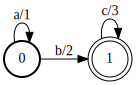
\includegraphics[scale=\dotscale]{figures/intersect_example_1}
    \end{subfigure}
    \begin{subfigure}[b]{0.68\textwidth}
        \centering
        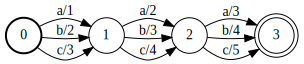
\includegraphics[scale=\dotscale]{figures/intersect_example_2}
    \end{subfigure}
    \caption{The automata on the left recognizes $a^*bc^*$, the automata on the
    right recognizes all three letter combinations of the alphabet $\{a, b,
    c\}$.}
    \label{fig:intersect_example_inputs}
\end{figure}

The intersection is given in figure~\ref{fig:intersect_example}. The
intersected graph accepts the sequences $aab$, $abc$, and $bcc$ which are
the only sequences accepted by both inputs.

\begin{figure}
    \centering
    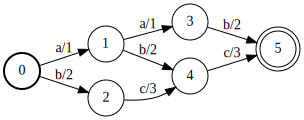
\includegraphics[scale=\dotscale]{figures/intersect_example}
    \caption{The intersection of the graphs in
    figure~\ref{fig:intersect_example_inputs} accepts the strings $aab$, $abc$,
    and $bcc$.}
    \label{fig:intersect_example}
\end{figure}
\end{proof}

\subsection{Compose}

The composition is a straightforward generalization of the intersection from
acceptors to transducers. Assume the first inpuut graph transduces the sequence
$\vx$ to the string $\vy$ and the second graph transduces $\vy$ to $\vz$. Then
the composed graph transduces $\vx$ to $\vz$.

From an implementation standpoint the compose and intersect algorithms are
almost identical. The two minor differences are 1) the way that labels are
matched in the input graphs and 2) the labels of the new arcs in the composed
graph. Arcs in a transducer have both input and output labels. We match the
output arc label from the first graph to the input arc label from the second
graph. This means that compose, unlike intersect, is not commutative, since the
order of the two graphs makes a difference.

The input label of a new arc in the composed graph is the input label of the
corresponding arc in the first input graph. The output label of a new arc in
the composed graph is the output label of the corresponding arc in the second
input graph. For example, assume we have two arcs, the first with label
$x_1\!:\!x_2$, and the second with label $y_1\!:\!y_2$. If $x_2 = y_1$, then
the arcs are considered a match. The new arc will have the label $x_1\!:\!y_2$.

Think of matrix mutiplication as an analogy or mnemonic device. When
multiplying two matrices they have to match on the inner dimension, and the
dimensions of the output matrix are the outer dimensions. In the same way the
inner labels of the two arcs must match and the resulting arc labels are the
outer labels of the two input arcs.

\begin{example}
Compute the composition of the two graphs in
figure~\ref{fig:compose_example_inputs}.
\end{example}

\begin{figure}
    \centering
    \begin{subfigure}[b]{0.3\textwidth}
        \centering
        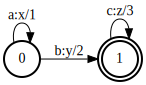
\includegraphics[scale=\dotscale]{figures/compose_example_1}
    \end{subfigure}
    \begin{subfigure}[b]{0.68\textwidth}
        \centering
        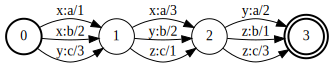
\includegraphics[scale=\dotscale]{figures/compose_example_2}
    \end{subfigure}
    \caption{Two transducers for which we would like to compute the composition.}
    \label{fig:compose_example_inputs}
\end{figure}

\begin{proof}[\unskip\nopunct]
The composition is given in figure~\ref{fig:compose_example}. As an example,
the first input graph transduces $abc$ to $xyz$ and the second input
transduces $xyz$ to $abb$, $abc$, $bbb$, and $bbc$. Thus, the composed
graph should transduce $abc$ to all four of $abb$, $abc$, $bbb$, and $bbc$.
You can verify this in the graph in figure~\ref{fig:compose_example}.

\begin{figure}
    \centering
    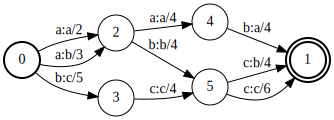
\includegraphics[scale=\dotscale]{figures/compose_example}
    \caption{The composition of the two graphs from
    figure~\ref{fig:compose_example_inputs}.}
    \label{fig:compose_example}
\end{figure}

\end{proof}

\subsubsection{Intersection and Composition with $\epsilon$}
\label{sec:epsilon_intersect}

The basic implementation of intersection and composition we have discussed so
far doesn't extend to $\epsilon$ transitions. Allowing $\epsilon$ transitions
in these algorithms makes them more complicated. In this section I will
illustrate the challenges with the naive approach and sketch at a high-level
how to actually include $\epsilon$ transitions in the algorithms.

First, consider the simpler case when only the first input graphs has
$\epsilon$ transitions. In this case, whenever we encounter an outgoing
$\epsilon$ transition from a state in the first graph we can optionally
traverse it without matching a corresponding arc in the second graph. Consider
the subgraphs in figure~\ref{fig:epsilon_intersect}.

\begin{figure}
    \centering
    \begin{subfigure}{0.32\textwidth}
        \centering
        \includegraphics[scale=\dotscale]{figures/epsilon_intersect_1}
    \end{subfigure}
    \begin{subfigure}{0.32\textwidth}
        \centering
        \includegraphics[scale=\dotscale]{figures/epsilon_intersect_2}
    \end{subfigure}
    \begin{subfigure}{0.32\textwidth}
        \centering
        \includegraphics[scale=\dotscale]{figures/epsilon_intersect}
    \end{subfigure}
    \caption{The graph on the left has an $\epsilon$ transition. Computing the
    intersection of the left and middle graph results in the graph on the
    right. The $\epsilon$ transition can be followed without consuming an input
    in the middle graph.}
    \label{fig:epsilon_intersect}
\end{figure}

Suppose we are currently looking for outgoing arcs with matching labels from
the state $(0, 0)$. When we find a matching pair, we add the new state to the
intersected graph and add a corresponding arc. In the $\epsilon$-free case, we
only explore the arc's with label $a$. The state $(1, 1)$ is added to the
intersected graph and the queue to be explored. The state $(0, 0)$ is connected
to the state $(1, 1)$ with an arc with label $a$ and weight $2$.

Since state $0$ in the first graph has an outgoing $\epsilon$, we can
optionally traverse it without traversing any arc in the second graph. In this
case, we add the state $(2, 0)$ to the intersected graph and to the queue to be
explored. We also add an arc from the state $(0, 0)$ to the state $(2, 0)$ in
the intersected graph with a label $\epsilon$ and a weight of $2$.

\begin{example}
Compute the intersection of the two graphs in
figure~\ref{fig:epsilon_intersect_example_inputs}.
\end{example}

\begin{figure}
    \centering
    \begin{subfigure}[b]{0.48\textwidth}
        \centering
        \includegraphics[scale=\dotscale]{figures/epsilon_intersect_example_1}
    \end{subfigure}
    \begin{subfigure}[b]{0.48\textwidth}
        \centering
        \includegraphics[scale=\dotscale]{figures/epsilon_intersect_example_2}
    \end{subfigure}
    \caption{An example of two acceptors for which we would like to compute the
    intersection. The acceptor on the left has an $\epsilon$ transition.}
    \label{fig:epsilon_intersect_example_inputs}
\end{figure}

\begin{proof}[\unskip\nopunct]
The intersected graph is in figure~\ref{fig:epsilon_intersect_example}. The
$\epsilon$ transition is included for clarity, though it could be removed
and states $1$ and $2$ collapsed yielding an equivalent graph.

\begin{figure}
    \centering
    \includegraphics[scale=\dotscale]{figures/epsilon_intersect_example}
    \caption{The intersection of the two graphs in
    figure~\ref{fig:epsilon_intersect_example_inputs}.}
    \label{fig:epsilon_intersect_example}
\end{figure}

\end{proof}

The trickier case to handle is when both graphs have $\epsilon$ transitions. If
we optionally explore outgoing $\epsilon$ arcs in each graph, then we will end
up with too many paths in the intersection. Suppose we are given the two graphs
in figure~\ref{fig:epsilon_intersect_both_inputs}, each of which has an
$\epsilon$ transition.

\begin{figure}
    \centering
    \begin{subfigure}[b]{0.48\textwidth}
        \centering
        \includegraphics[scale=\dotscale]{figures/epsilon_intersect_both_1}
    \end{subfigure}
    \begin{subfigure}[b]{0.48\textwidth}
        \centering
        \includegraphics[scale=\dotscale]{figures/epsilon_intersect_both_2}
    \end{subfigure}
    \caption{Two acceptors, both of which have $\epsilon$ transitions.}
    \label{fig:epsilon_intersect_both_inputs}
\end{figure}

If we compute the intersection of the two graphs in
figure~\ref{fig:epsilon_intersect_both_inputs}, optionally following $\epsilon$
transitions as we encounter them, then we end up with the graph in
figure~\ref{fig:epsilon_intersect_both}.

\begin{figure}
    \centering
    \includegraphics[scale=\dotscale]{figures/epsilon_intersect_both}
    \caption{An incorrect composition of the two graphs in
    figure~\ref{fig:epsilon_intersect_both_inputs}. Naively following
    $\epsilon$ transitions as we encounter them when computing the intersection
    results in an incorrect graph. The graph admits too many paths for the
    sequence $ab$, and hence the score of that sequence is incorrect.}
    \label{fig:epsilon_intersect_both}
\end{figure}

The language of this graph is correct. It accepts the string $ab$ which is the
only string in the intersection. However, the weight it assigns to the string
$ab$ is incorrect. Each individual path has the correct weight, but there are
three paths for $ab$. The final weight will receive three contributions, one
from each path, instead of a single contribution from one path. The solution to
this problem is to choose only one of the three paths and avoid the inadvertant
redundancy. For example we could keep the bottom path and ignore the top two as
in the graph in figure~\ref{fig:epsilon_intersect_both_correct}.

\begin{figure}
    \centering
    \includegraphics[scale=\dotscale]{figures/epsilon_intersect_both_correct}
    \caption{Correctly accounting for $\epsilon$ transitions when intersecting
    the two graphs in figure~\ref{fig:epsilon_intersect_both_inputs}. Notice
    that only one of the three resultant paths should be retained in the
    intersected graph.}
    \label{fig:epsilon_intersect_both_correct}
\end{figure}

\subsection{Forward and Viterbi}

The forward score and the Viterbi score take a graph as input and return a
single scalar result. The \emph{forward score} is the accumulation of the
weights of all possible paths from any start state to any accept state in the
graph. The weight of the highest scoring path is the \emph{Viterbi score}, and the
path itself is the \emph{Viterbi path}.

\begin{center}
\begin{tabular}{p{.95\textwidth}}
\midrule\\
\vspace{-10mm}
\subsubsection{Aside: Shortest Distance}
In some descriptions of weighted automata, the forward and Viterbi score are
introduced as shortest distance algorithms under a respective semiring. The
forward score corresponds to the log semiring and the Viterbi score corresponds
to the tropical semiring. This is a more general perspective, and useful if you
intend to use other semirings. However, we only need the log and tropical
semirings in all of the applications we study, so we will restrict the
description to the more specific forward and Viterbi score.
\\\midrule\\
\end{tabular}
\end{center}

Let's start with a couple of examples to show exactly what we are trying to
compute, then we will go through a more general algorithm for forward and
Viterbi scoring. For the forward and Viterbi score, we will restrict the graphs
to be acyclic, meaning no self-loops or cycles. Under certain technical
conditions a graph with cycles can admit a computable forward and Viterbi
score, but we won't discuss these cases as they don't come up often in
machine-learning applications.

\begin{figure}
    \centering
    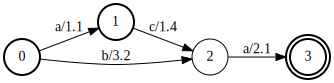
\includegraphics[scale=\dotscale]{figures/score_example}
    \caption{An acceptor with three paths from the start states $0$ and $1$ to
    the accept state $3$.}
    \label{fig:score_example}
\end{figure}

The graph in figure~\ref{fig:score_example} has three possible paths from the
start states to the accept state. The paths and their scores are:

\begin{itemize}
    \item State sequence $0 \rightarrow 1 \rightarrow 2 \rightarrow 3$ with
        score 4.6
    \item State sequence $0 \rightarrow 2 \rightarrow 3$ with score 5.3
    \item State sequence $1 \rightarrow 2 \rightarrow 3$ with score 3.5
\end{itemize}

The Viterbi score is the maximum over the individual path scores, in this case
$\max\{4.6, 5.3, 3.5\} = 5.3$. The Viterbi path is the sequence of labels which
correspond to the arcs contributing to the Viterbi score. We represent the
Viterbi path as a simple linear graph as in figure~\ref{fig:viterbi_path}. Note
the Viterbi path may not be unique--multiple paths could all attain the Viterbi
score. The forward score is the \emph{log-sum-exp} over all the path scores, in
this case $\LSE(4.6, 5.3, 3.5) = 5.81$. The forward score will always be larger
than the Viterbi score. However, the two will converge as the difference
between Viterbi score and the second highest scoring path increases.

\begin{figure}
    \centering
    \includegraphics[scale=\dotscale]{figures/viterbi_path}
    \caption{The Viterbi path for the graph in figure~\ref{fig:score_example}.
    The score of the Viterbi path is the Viterbi score, in this case $5.3$.}
    \label{fig:viterbi_path}
\end{figure}

We computed the forward and Viterbi score by listing all possible paths,
computing their individual weights, and then accumulating either with the
$\max$ or the $LSE$ operations. This approach won't scale to larger graphs
because the number of paths can grow combinatorially. Instead, we will use a
much more efficient dynamic programming algorithm which works for both the
forward and Viterbi score.

The dynamic programming algorithm relies on the following recurions. Consider a
state $v$ and let $e_i$ for $i=1, \ldots, k$ be the set of arcs for which $v$
is the destination node. For a given arc $e$ we let $\textrm{source}(e)$ denote
the source node for that arc. The score of all paths which start at a start
state and terminate at node $v$ can be constructed from the score of all paths
which start at a start state and terminate at the state $\textrm{source}(e_i)$
and the arc weight $w(e_i)$ for $i=1\ldots, k$. For the Viterbi score, the
recursion is:
$$
s_v = \max_{i=1}^k \left( s_{\textrm{source}(e_i)} + w(e_i) \right),
$$
where $s_v$ is the score of all paths starting at a start state terminating at
state $v$, and $s_{\textrm{source}(e_i)}$ is the score of all paths starting at
a start state terminating at state $\textrm{source}(e_i)$. The recursion is
shown graphically in figure~\ref{fig:viterbi_recursion}. In
figure~\ref{fig:viterbi_recursion}, the Viterbi score of state $3$ is the
maximum over the weight plus the source node score for all incoming arcs.

\begin{figure}
    \centering
    \includegraphics[scale=\dotscale]{figures/viterbi_recursion}
    \caption{A graphical depiction of the recursion for computing the Viterbi
    score.}
    \label{fig:viterbi_recursion}
\end{figure}

The overall Viterbi score is the max of the Viterbi scores over the accept
states, $\max_a s_a$ where $a$ is an accept state.

The forward score uses the exact same recursion but with an $\LSE$ in place of
the $\max$:
$$
s_v = \LSE_{i=1}^k \left( s_{\textrm{source}(e_i)} + w(e_i) \right),
$$
and the final score is $\LSE_a s_a$.

For both the forward and Viterbi score, the recursion works because the $\LSE$
and $\max$ operations admit a simple decomposition of the score for all paths
terminating at a given state. Suppose, as in the graph in
figure~\ref{fig:dp_recursion}, we have a state $v$ for which we want to compute
the score $s_v$. Suppose also that $v$ has only one incoming arc from state
$u$. Three paths from a start state terminate at state $u$ with the given
scores $p_1$, $p_2$, and $p_3$. We can extend each of the three paths from $u$
to $v$ by adding the arc between them, so there are three paths terminating at
$v$ as well.

\begin{figure}
    \centering
    \includegraphics[scale=\dotscale]{figures/dp_recursion}
    \caption{The recursion in computing the Viterbi and forward score works
    because the score $s_v$ at state $v$ can be computed from the weight $w$
    and the score $s_u$ at state $u$.}
    \label{fig:dp_recursion}
\end{figure}

First, suppose we want to compute the Viterbi score at $v$. The Viterbi score
is the maximum of the weights of all three paths terminating at $v$, namely
$s_v = \max \{w + p_1, w + p_2, w + p_3\}$. We can also compute the Viterbi
score $s_v$ from the Viterbi score, $s_u$, of paths terminating at $u$. In this
case $s_v = w + s_u$. This is the recursion we used above but for simplicity
with only one incoming arc to $v$. The two ways of computing $s_v$ are
equivalent:
\begin{align*}
s_v &= w + s_u \\
    &= w + \max \{p_1, p_2, p_3 \} \\
    &= \max \{w + p_1, w + p_2, w + p_3\} \\
    &= s_v.
\end{align*}

The same decomposition works for the forward score and the $\LSE$ operation:
\begin{align*}
s_v &= w + s_u  \\
    &= w + \log \left(e^{p_1} + e^{p_2} + e^{p_3}\right) \\
    &= \log e^w + \log \left(e^{p_1} + e^{p_2} + e^{p_3}\right) \\
    &= \log e^w \left(e^{p_1} + e^{p_2} + e^{p_3}\right) \\
    &= \log \left(e^{w + p_1} + e^{w + p_2} + e^{w + p_3}\right) \\
    &= s_v
\end{align*}

For simplicity, we assume only three paths terminating at $u$ and one arc
incoming to $v$. The argument is easily extended to an arbitrary number of
paths and arcs.

\subsubsection{Viterbi Path}

A Viterbi path is a path for which the Viterbi score is attained. We can
compute one of the Viterbi paths with a straightforward extension of the
Viterbi scoring algorithm. At each state when we compute the score, we also
maintain a backpointer to the arc which resulted in the maximum score. When the
algorithm terminates, we can trace the backpointers to the start state and
extract the Viterbi path.

An example of this can be seen in the graph in
figure~\ref{fig:viterbi_path_back}.

\begin{figure}
    \centering
    \includegraphics[scale=\dotscale]{figures/viterbi_path_back}
    \caption{Each state is labeled with the state label and viterbi score from
    the start state up to that state. The red arrows indicate the arc which is
    part of the Viterbi path up to the given state. The complete Viterbi path
    can be found by following red arcs back from the accept state.}
    \label{fig:viterbi_path_back}
\end{figure}

Each state in the graph is labeled with the Viterbi score over all paths
terminating at that state. The red arcs are the arcs which result in the
maximum score for the state that they point to. In order to compute the Viterbi
path, we trace the red arcs back from the accept state. In this case the
Viterbi path state sequence is $0 \rightarrow 2 \rightarrow 4 \rightarrow 6$
with arc labels $b$, $c$, and $b$.

\begin{example}
Compute the Viterbi path of the graph in
figure~\ref{fig:viterbi_path_example_input}.
\end{example}

\begin{figure}
    \centering
    \includegraphics[scale=\dotscale]{figures/viterbi_path_example_input}
    \caption{An example acceptor for which we would like to compute the Viterbi
    path.}
    \label{fig:viterbi_path_example_input}
\end{figure}

\begin{proof}[\unskip\nopunct]
The Viterbi path is shown in  figure~\ref{fig:viterbi_path_example}.
\end{proof}

\begin{figure}
    \centering
    \includegraphics[scale=\dotscale]{figures/viterbi_path_example}
    \caption{The Viterbi path of the graph in
    figure~\ref{fig:viterbi_path_example_input}.}
    \label{fig:viterbi_path_example}
\end{figure}
